\documentclass[11pt]{article}
\usepackage{amsmath}
\usepackage{amsfonts}
\usepackage{amsthm}
\usepackage{graphicx}
\usepackage{amssymb}
\usepackage{slashed}
\usepackage{listings}
\usepackage{color}

%----------------------------------------------------------------------------------------------------------------------------------------
% Defines various parameters for lstlisting for code snippets
\definecolor{dkgreen}{rgb}{0,0.6,0}
\definecolor{gray}{rgb}{0.5,0.5,0.5}
\definecolor{mauve}{rgb}{0.58,0,0.82}
\definecolor{highlight}{RGB}{255,251,204}

\lstset{frame=tb,
  language=R,
  backgroundcolor=\color{highlight},
  aboveskip=3mm,
  belowskip=3mm,
  showstringspaces=false,
  columns=flexible,
  basicstyle={\small\ttfamily},
  numbers=none,
  numberstyle=\tiny\color{gray},
  keywordstyle=\color{blue},
  commentstyle=\color{dkgreen},
  stringstyle=\color{mauve},
  breaklines=true,
  breakatwhitespace=true,
  tabsize=3}
%----------------------------------------------------------------------------------------------------------------------------------------

%----------------------------------------------------------------------------------------------------------------------------------------
% Set page geometry parameters
\textwidth = 6.5 in
\textheight = 8.5 in
\oddsidemargin = 0.0 in
\evensidemargin = 0.0 in
\topmargin = 0.0 in
\headheight = 0.0 in
\headsep = 0.5 in
\parskip = 0.2in
\parindent = 0.0in
%----------------------------------------------------------------------------------------------------------------------------------------

%----------------------------------------------------------------------------------------------------------------------------------------
%Defines macros for some mathematical tools.  Probably not useful here.
\providecommand{\abs}[1]{\lvert#1\rvert}
\providecommand{\norm}[1]{\lvert\lvert#1\rvert\lvert}
\providecommand{\inner}[2]{\langle#1 , #2\rangle}
\providecommand{\unionover}[3]{ {\underset{#1 \in #2}{\bigcup}} {#3}}
\providecommand{\intover}[3]{ {\underset{#1 \in #2}{\bigcap}} {#3}}

\providecommand{\code}[1]{{\color{red}\ttfamily #1}}
%----------------------------------------------------------------------------------------------------------------------------------------
\begin{document}
\section*{Chapter 4}
\begin{enumerate}
%----------------------------------------------------------------------------------------------------------------------------------------
%----------------------------------------------------------------------------------------------------------------------------------------
\subsection*{Conceptual}
\item  Using a little bit of algebra, prove that
\begin{equation}
p(X)=\frac{e^{\beta_0+\beta_1 X}}{1+e^{\beta_0+\beta_1 X}}
\end{equation}
is equivalent to
\begin{equation}
\frac{p(X)}{1-p(X)}=e^{\beta_0+\beta_1 X}.
\end{equation}
In other words, the logistic function and logit representation for the logistic regression model are equivalent.

\begin{proof}
Let $p(X)=\frac{e^{\beta_0+\beta_1 X}}{1+e^{\beta_0+\beta_1 X}}$.  Thus
\begin{equation}
\begin{split}
\frac{p(X)}{1-p(X)}&=\frac{\frac{e^{\beta_0+\beta_1 X}}{1+e^{\beta_0+\beta_1 X}}}{1-\frac{e^{\beta_0+\beta_1 X}}{1+e^{\beta_0+\beta_1 X}}}\\
&=\frac{e^{\beta_0+\beta_1 X}}{1+e^{\beta_0+\beta_1 X}- e^{\beta_0+\beta_1 X}}\\
&=e^{\beta_0+\beta_1 X}\\
\end{split}
\end{equation}
Further, if $\frac{p(X)}{1-p(X)}=e^{\beta_0+\beta_1 X}$, then $p(X)=(1-p(X))e^{\beta_0+\beta_1 X}$.  Hence $p(X)(1+e^{\beta_0+\beta_1 X})=e^{\beta_0+\beta_1 X}$ and so $p(X)=\frac{e^{\beta_0+\beta_1 X}}{1+e^{\beta_0+\beta_1 X}}$.

Thus $p(X)=\frac{e^{\beta_0+\beta_1 X}}{1+e^{\beta_0+\beta_1 X}}$ if and only if $\frac{p(X)}{1-p(X)}=e^{\beta_0+\beta_1 X}$.
\end{proof}

\item It was stated in the text that classifying an observation to the class for which 
\begin{equation}
p_k(x)=\frac{\pi_k\frac{1}{\sqrt{2\pi}\sigma}\text{exp}{(-\frac{1}{2\sigma^2}(x-\mu_k)^2})}{\sum_{l=1}^K \pi_l\frac{1}{\sqrt{2\pi}\sigma}\text{exp}{(-\frac{1}{2\sigma^2}(x-\mu_l)^2})}
\end{equation}
is largest is equivalent to classifying an observation to the class for which 
\begin{equation}
\delta_k(x)=x\frac{\mu_k}{\sigma^2}-\frac{\mu_k^2}{2\sigma^2}+\log(\pi_k)
\end{equation}
is largest.  Prove this is the case.  In other words, under the assumption that observations in the $k$th class are drawn from a $N(\mu_k,\sigma^2)$ distribution, the Bayes' classifier assigns an observation to the class for which the discriminant function is maximized. 
\begin{proof}
Let $x$ be a fixed observation.  First suppose that $k$ maximizes the discriminant.  Thus $\delta_k(x)\geq\delta_i(x)$ for all $i$.  Thus since the exponential function is strictly increasing 
$\pi_k\exp{(x\frac{\mu_k}{\sigma^2}-\frac{\mu_k^2}{2\sigma^2})}\geq \pi_i\exp{(x\frac{\mu_i}{\sigma^2}-\frac{\mu_i^2}{2\sigma^2})}$ for all $i$.  Now since 
\begin{equation}
\frac{\exp(-\frac{1}{2\sigma^2}x^2)}{\sum_{l=1}^K \pi_l\frac{1}{\sqrt{2\pi}\sigma}\exp{(-\frac{1}{2\sigma^2}(x-\mu_l)^2})}>0,
\end{equation}
it follows that 
\begin{equation}
\frac{\pi_k\exp{(x\frac{\mu_k}{\sigma^2}-\frac{\mu_k^2}{2\sigma^2})}\exp(-\frac{1}{2\sigma^2}x^2)}{\sum_{l=1}^K \pi_l\frac{1}{\sqrt{2\pi}\sigma}\exp{(-\frac{1}{2\sigma^2}(x-\mu_l)^2})}\geq
\frac{\pi_i\exp{(x\frac{\mu_i}{\sigma^2}-\frac{\mu_i^2}{2\sigma^2})}\exp(-\frac{1}{2\sigma^2}x^2)}{\sum_{l=1}^K \pi_l\frac{1}{\sqrt{2\pi}\sigma}\exp{(-\frac{1}{2\sigma^2}(x-\mu_l)^2})}
\end{equation}
for all $i$ and thus 
\begin{equation}
\frac{\pi_k\exp((-\frac{1}{2\sigma^2})(x^2-2\mu_k x +\mu_k^2))}{\sum_{l=1}^K \pi_l\frac{1}{\sqrt{2\pi}\sigma}\exp{(-\frac{1}{2\sigma^2}(x-\mu_l)^2})}\geq\frac{\pi_i\exp((-\frac{1}{2\sigma^2})(x^2-2\mu_i x +\mu_i^2))}{\sum_{l=1}^K \pi_l\frac{1}{\sqrt{2\pi}\sigma}\exp{(-\frac{1}{2\sigma^2}(x-\mu_l)^2})}
\end{equation}
for all $i$.  Therefore $p_k(x)\geq p_i(x)$ for all $i$ and hence $k$ maximizes the posterior probability.

The reverse implication is similar.
\end{proof}
\item This problem relates to the QDA model, in which the observations within each class are drawn from a normal distribution with a class specific mean vector and a class specific covariance matrix.  We consider the simple case where $p=1$; i.e. there is only one feature.

Suppose that we have $K$ classes, and that if an observation belongs to the $k$th class then $X$ comes from a one dimensional normal distribution, $X\sim N(\mu_k,\sigma_k^2)$.  Recall that the density function for the one dimensional normal distribution is given by 
\begin{equation}
f_k(x)=\frac{1}{\sqrt{2\pi}\sigma_k}\exp{\left(-\frac{1}{2\sigma_k^2}(x-\mu_k)^2\right)}.
\end{equation}
Prove that in this case, the Bayes' classifier is not linear.  Argue that it is in fact quadratic.
\begin{proof}
Suppose that we have $K$ classes, and that if an observation belongs to the $k$th class then $X$ comes from a one dimensional normal distribution, $X\sim N(\mu_k,\sigma_k^2)$ and $p=1$.  Thus for each $k$ \begin{equation}
f_k(x)=\frac{1}{\sqrt{2\pi}\sigma_k}\exp{\left(-\frac{1}{2\sigma_k^2}(x-\mu_k)^2\right)}.
\end{equation}
and hence by Bayes' theorem 
\begin{equation}
p_k(x)=\frac{\pi_k\frac{1}{\sqrt{2\pi}\sigma_k}\text{exp}{(-\frac{1}{2\sigma_k^2}(x-\mu_k)^2})}{\sum_{l=1}^K \pi_l\frac{1}{\sqrt{2\pi}\sigma_l}\text{exp}{(-\frac{1}{2\sigma_l^2}(x-\mu_l)^2})}
\end{equation}
for each $k$.  Now taking the $\log$ of both sides we find
\begin{equation}
\log(p_k(x))=\log\left(\pi_k\frac{1}{\sqrt{2\pi}\sigma_k}\text{exp}\left(-\frac{1}{2\sigma_k^2}(x-\mu_k)^2\right)\right)-\log\left(\sum_{l=1}^K \pi_l\frac{1}{\sqrt{2\pi}\sigma_l}\text{exp}\left(-\frac{1}{2\sigma_l^2}(x-\mu_l)^2\right)\right)
\end{equation}
 and thus
 \begin{equation}
 \begin{split}
 \delta_k(x)&= \log(p_k(x)) + \log\left(\sum_{l=1}^K \pi_l\frac{1}{\sqrt{2\pi}\sigma_l}\text{exp}\left(-\frac{1}{2\sigma_l^2}(x-\mu_l)^2\right)\right)\\
 &=\log\left(\pi_k\frac{1}{\sqrt{2\pi}\sigma_k}\text{exp}\left(-\frac{1}{2\sigma_k^2}(x-\mu_k)^2\right)\right)\\
 &=\log(\pi_k)-\log(\sqrt{2\pi}\sigma_k)-\frac{1}{2\sigma_k^2}(x-\mu_k)^2\\
  &=\log(\pi_k)-\log(\sqrt{2\pi}\sigma_k)-\frac{1}{2\sigma_k^2}x^2+\frac{1}{\sigma_k^2}x\mu_k+\frac{1}{2\sigma_k^2}\mu_k^2.\\
 \end{split}
 \end{equation}
 Note that now since the variances are class specific the $\frac{1}{2\sigma_k^2}x^2$ term depends on $k$ as well as $x$ and hence cannot be included as part of the descriminant.  Thus $\delta_k(x)$ is quadratic in $x$. 
\end{proof}

\item When the number of features $p$ is large, there tends to be a deterioration in the performance of KNN and the other local approaches that perform prediction using only observations that are near the test observation for which a prediction must be made.  This phenomenon is known as the curse of dimensionality, and it ties into the fact that non-parametric approaches often perform poorly when $p$ is large.  We will now investigate this curse.
\begin{enumerate}
\item Suppose that we have a set of observations, each with measurements on $p=1$ feature, $X$.  We assume that $X$ is uniformly distributed on $[0,1]$.  Associated with each observation is a response value.  Suppose we wish to predict a test observation's response using only observations that are within $10\%$ of the range of $X$ closest to that test observation.  For instance, in order to predict the response for a test observation with $X=0.6$, we will use observations in the range $[0.55,0.65]$.  On average, what fraction of the available observations will we use to make the prediction?

Note that the length of such an interval is 0.1.  Thus we would expect a uniform random variable on $[0,1]$ to lie in such an interval with probability $0.1/1=0.1$.  Thus on average we would be using $10\%$ of the available observations to make the prediction. 

\item Now suppose that we have a set of observations, each with measurements on $p=2$ features, $X_1$ and $X_2$.  We assume that $(X_1,X_2)$ are uniformly distributed on $[0,1]\times[0,1]$.  We wish to predict an observation's response using only observations that are within $10\%$ of the range of $X_1$ and within $10\%$ of the range of $X_2$ closest to that test observation.  For instance, in order to predict the response for a test observation with $X_1=0.6$ and $X_2=0.35$, we will use observations in the range $[0.55,0.65]$ for $X_1$ and in the range $[0.3,0.4]$ for $X_2$.  On average, what fraction of the available observations will we use to make the prediction?

Note that the area of such a square is $0.1^2=0.01$.  Thus we would expect a uniform random variable on $[0,1]\times[0,1]$ to lie in such a square with probability $0.01/1=0.01$.  Thus on average we would be using $1\%$ of the available observations to make the prediction. 

\item Now suppose that we have a set of observations on $p=100$ features.  Again the observations are uniformly distributed on each feature, and again each feature ranges from 0 to 1.  We wish to predict a test observation's response using observations within $10\%$ of each features range that is closest to that test observation.  What fraction of the available observations will we use to make the prediction?

Note that the volume of such a hypercube is $0.1^100=10^{-100}$.  Thus we would expect a uniform random variable on the unit 100 dimensional hypercube to lie in such a hypercube with probability $10^{-100}/1=10^{-100}$.  Thus on average we would be using $1/10^{100}$ of the available observations to make the prediction.

\item Using your answers to (a)-(c), argue that a drawback of KNN when $p$ is large is that there are very few training observations ``near" any given test observation. 

From the above we note that the fraction of observations within a given distance of a predictor tends to zero as the number of features increases.

\item Now suppose that we wish to make a prediction for a test observation by creating a $p$ dimensional hypercube centered around the test observation that contains, on average, $10\%$ of the training observations.  For $p=1,2,$ and $100$, what is the length of each side of the hypercube?  Comment on your answer.    

Note that the volume of a $p$ dimensional hypercube with side length $a$ is $a^p$.  Thus the volume of the unit hypercube is 1 and the probability that a uniform random variable will lie in a given hypercube of side length $a$ for $0<a\leq 1$ is $\frac{a^p}{1}=a^{p}$.  Hence, in order for such a hypercube to contain $1/b$ of the available training observations, in expectation,  we require that $1/b=a^{p}$.  That is we require $a=(\frac{1}{b})^{1/p}$.

Thus for $b=10$ and $p=1$ we require $a=\frac{1}{10}$.  For $b=10$ and $p=2$ we require $a=\frac{1}{\sqrt{10}}\approx0.316$.  For $b=10$ and $p=100$ we require $a=\frac{1}{10^\frac{1}{100}}\approx0.977$.  In particular, for any fixed $b>1$ we have $\displaystyle\lim_{p\to\infty} a(p)=1$.
\end{enumerate}

\item We now examine the differences between LDA and QDA.
\begin{enumerate}
\item If the Bayes decision boundary is linear, do we expect LDA or QDA to perform better on the training set? On the test set?

We would expect QDA to perform better on the test set since it is a more flexible model.  However we would expect LDA to perform better on the test set in this situation as the flexibility in QDA will cause it to overfit the data.\\

\item If the Bayes decision boundary is non-linear, do we expect LDA or QDA to perform better on the training set? On the test set?

In this situation we would expect QDA to perform better on both the training and test sets.  LDA will have too much bias.\\

\item In general, as the sample size $n$ increases, do we expect the test prediction accuracy of QDA relative to LDA to improve, decline or be unchanged? Why?

As the sample size increases we expect the test prediction accuracy of QDA to improve relative to LDA.  Since LDA is a high bias model, it's test prediction accuracy should remain relatively constant past a certain amount of data.  Since QDA is a lower bias model, more data will tend to decrease the higher variance and hence increase prediction accuracy.\\   

\item True or False: Even if the Bayes decision boundary for a given problem is linear, we will probably achieve a superior test error rate using QDA rather than LDA because QDA is flexible enough to model a linear decision boundary.  Justify your answer.

This is false.  If the Bayes decision boundary is linear than the increased flexibility of QDA may cause it to significantly overfit the data.  While QDA's training error rate will be better, the overfitting will cause the model to not generalize well to new observations.  As noted above, the overfitting will decrease as the training sample size increases but will always be present. \\
\end{enumerate}

\item Suppose we collect data for a group of students in a statistics class with variables $X_1=$ hours studied, $X_2=$ undergrad GPA, and $Y=$receive and A.  We fit a logistic regression and produce estimated coefficient, $\hat\beta_0=-6$, $\hat\beta_1=0.05$, $\hat\beta_2=1$.
\begin{enumerate}
\item Estimate the probability that a a student who studies for 40 hr. and has an undergrad GPA of 3.5 gets an A in the class.

From the fitted model,
\begin{equation}
p(40,3.5)=\frac{e^{-6+0.05(40)+(3.5)}}{1+e^{-6+0.05(40)+(3.5)}}\approx 0.37754
\end{equation}
Such a student has a predicted probability of 37.75\% of getting an A.

\item How many hours would the student in part (a) need to study to have a 50\% chance of getting an A in the class? 

To have a 50\% chance of an A, we would need 
\begin{equation}
0.5=\frac{e^{-6+0.05x+3.5}}{1+e^{-6+0.05x+3.5}}
\end{equation}
where $x$ is the number of hours studied.  Thus $x=50$.
\end{enumerate}

\item Suppose that we wish to predict whether a given stock will issue a dividend this year (``Yes" or ``No") based on $X$, last years percent profit.  We examine a large number of companies and discover that the mean value of $X$ for companies that issued a dividend was $\bar X=10$, while the mean value for those that didn't was $\bar X=0$.  In addition, the variance of $X$ for these two sets of companies was $\hat\sigma^2=36$.  Finally, $80\%$ of companies issued dividends.  Assuming that $X$ follows a normal distribution, predict the probability that a company will issue a dividend this year given that its percentage profit was $X=4$ last year.

Note that by Bayes' theorem we have
\begin{equation}
P(\text{Yes}|X=4)=\frac{P(\text{Yes})P(X=4|\text{Yes})}{P(X=4)}.
\end{equation}

Now by assumption $P(X=4|\text{Yes})\sim N(10,36)$ and $P(\text{Yes})=.8$
\begin{equation}
\begin{split}
P(\text{Yes}|X=4)&=\frac{P(\text{Yes})\frac{1}{\sqrt{2\pi}\sigma}\exp\left(-\frac{1}{2\sigma^2}(x-\mu_k)^2\right)}{P(\text{Yes})\frac{1}{\sqrt{2\pi}\sigma}\exp\left(-\frac{1}{2\sigma^2}(x-\mu_k)^2\right)+ P(\text{No})\frac{1}{\sqrt{2\pi}\sigma}\exp\left(-\frac{1}{2\sigma^2}(x-\mu_k)^2\right)}\\
&=\frac{0.8\cdot\exp\left(-\frac{1}{2\cdot 36}(4-10)^2\right)}{0.8\cdot\exp\left(-\frac{1}{2\cdot 36}(4-10)^2\right) + 0.2\cdot\exp\left(-\frac{1}{2\cdot 36}(4-0)^2\right)}\\
&\approx .75185
\end{split}
\end{equation}
Thus the is a $75.2\%$ probability that the company will issue a dividend.

\item Suppose that we take a data set, divide it into equally-sized training and test sets, and then try out two different classification procedures.  First we use logistic regression and get an error rate of $20\%$ on the training data and $30\%$ on the test data.  Next we use 1-nearest neighbors and get an average error rate of $18\%$.  Based on these results, which method should we prefer to use for classification of new observations? Why?

Based on these results we would prefer logistic regression.  This is because 1-nearest neighbors will have perfect accuracy on the training set and so an 18\% average error corresponds to a 36\% error rate on the test set (since the training and test sets are the same size). \\

\item This problem has to do with odds.
\begin{enumerate}
\item On average, what fraction of people with an odds of $0.37$ of defaulting on their credit card payment will in fact default?
If a person has on odds of $0.37$ of defaulting, then the probability of defaulting, $p$, satisfies
\begin{equation}
\frac{p}{1-p}=0.37
\end{equation}
and hence 
\begin{equation}
p=\frac{0.37}{1+0.37}\approx 0.27.
\end{equation}
Thus we would expect $27\%$ of such people to default.\\
\item Suppose that an individual has a $16\%$ chance of defaulting on her credit card payment.  What are the odds that she will default?
If a person has a probability of $0.16$ of defaulting, then the odds of defaulting, $p$, are
\begin{equation}
\frac{p}{1-p}=\frac{0.16}{1-0.16}\approx0.19.
\end{equation}
\end{enumerate}

\subsection*{Applied}
\item This question should be answered using the \code{Weekly} data set, which is part of the \code{ISLR} package.  This data is similar in nature to the \code{Smarket} data from this chapter's lab, except that it contains 1089 weekly returns for 21 years, from the beginning of 1990 to the end of 2010.
\begin{enumerate}
\item Produce some numerical and graphical summaries of the \code{Weekly} data.  Do there appear to be any patterns?
\begin{lstlisting}
> library(ISLR)
> attach(Weekly)
> summary(Weekly)
      Year           Lag1               Lag2               Lag3         
 Min.   :1990   Min.   :-18.1950   Min.   :-18.1950   Min.   :-18.1950  
 1st Qu.:1995   1st Qu.: -1.1540   1st Qu.: -1.1540   1st Qu.: -1.1580  
 Median :2000   Median :  0.2410   Median :  0.2410   Median :  0.2410  
 Mean   :2000   Mean   :  0.1506   Mean   :  0.1511   Mean   :  0.1472  
 3rd Qu.:2005   3rd Qu.:  1.4050   3rd Qu.:  1.4090   3rd Qu.:  1.4090  
 Max.   :2010   Max.   : 12.0260   Max.   : 12.0260   Max.   : 12.0260  
      Lag4               Lag5              Volume            Today          Direction 
 Min.   :-18.1950   Min.   :-18.1950   Min.   :0.08747   Min.   :-18.1950   Down:484  
 1st Qu.: -1.1580   1st Qu.: -1.1660   1st Qu.:0.33202   1st Qu.: -1.1540   Up  :605  
 Median :  0.2380   Median :  0.2340   Median :1.00268   Median :  0.2410             
 Mean   :  0.1458   Mean   :  0.1399   Mean   :1.57462   Mean   :  0.1499             
 3rd Qu.:  1.4090   3rd Qu.:  1.4050   3rd Qu.:2.05373   3rd Qu.:  1.4050             
 Max.   : 12.0260   Max.   : 12.0260   Max.   :9.32821   Max.   : 12.0260
 
> plot(Weekly)
\end{lstlisting}
\begin{center}
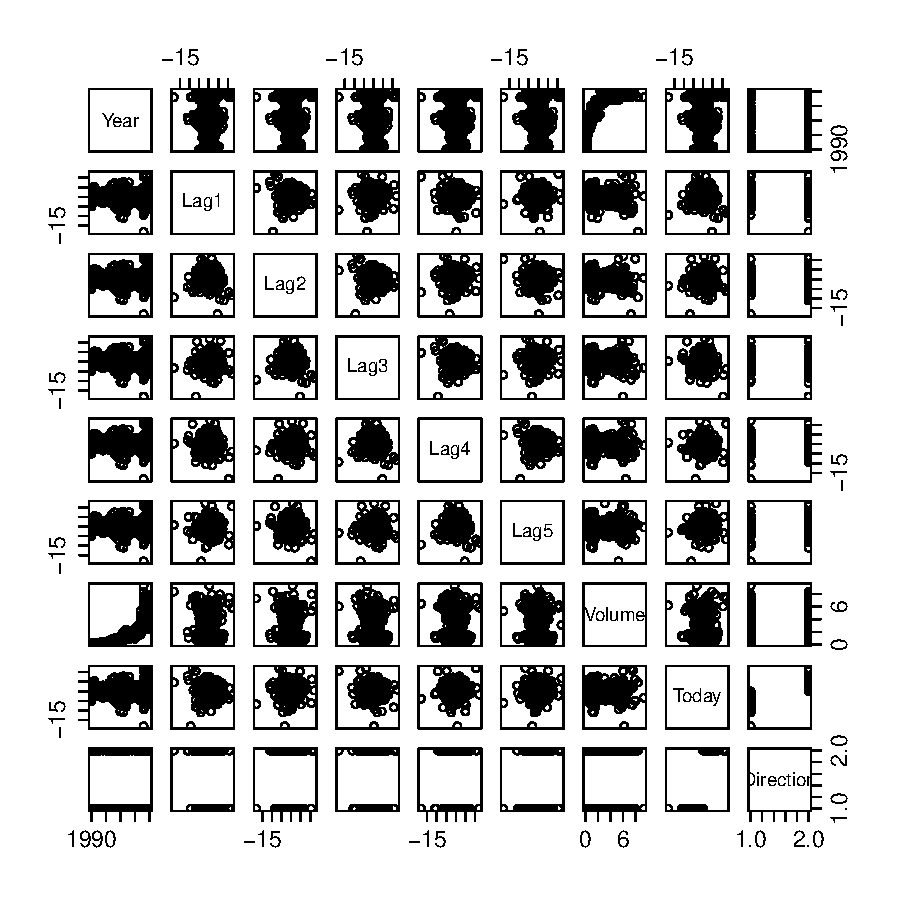
\includegraphics[scale=.75]{plot1.pdf}
\end{center}
\begin{lstlisting}
> cor(Weekly[1:8])
              Year         Lag1        Lag2        Lag3         Lag4         Lag5
Year    1.0000000 -0.032289274 -0.03339001 -0.03000649 -0.031127923 -0.030519101
Lag1   -0.03228927  1.000000000 -0.07485305  0.05863568 -0.071273876 -0.008183096
Lag2   -0.03339001 -0.074853051  1.00000000 -0.07572091  0.058381535 -0.072499482
Lag3   -0.03000649  0.058635682 -0.07572091  1.00000000 -0.075395865  0.060657175
Lag4   -0.03112792 -0.071273876  0.05838153 -0.07539587  1.000000000 -0.075675027
Lag5   -0.03051910 -0.008183096 -0.07249948  0.06065717 -0.075675027  1.000000000
Volume  0.84194162 -0.064951313 -0.08551314 -0.06928771 -0.06107461 -0.058517414
Today  -0.03245989 -0.075031842  0.05916672 -0.07124364 -0.007825873  0.011012698
            Volume        Today
Year    0.84194162 -0.032459894
Lag1   -0.06495131 -0.075031842
Lag2   -0.08551314  0.059166717
Lag3   -0.06928771 -0.071243639
Lag4   -0.06107462 -0.007825873
Lag5   -0.05851741  0.011012698
Volume  1.00000000 -0.033077783
Today  -0.03307778  1.000000000
\end{lstlisting}
Other than a correlation between volume and year, there does not appear to be any discernible patterns in the data.\\

\item Use the full data set to perform a logistic regression with \code{Direction} as the response and the five lag variables plus \code{Volume} as the predictors.  Use the summary function to print the results.  Do any of the predictors appear to be statistically significant?  If so, which ones?
\begin{lstlisting}
> glm.fit=glm(Direction~Lag1+Lag2+Lag3+Lag4+Lag5+Volume, data=Weekly, family=binomial)
> summary(glm.fit)

Call:
glm(formula = Direction ~ Lag1 + Lag2 + Lag3 + Lag4 + Lag5 + 
    Volume, family = binomial, data = Weekly)

Deviance Residuals: 
    Min       1Q   Median       3Q      Max  
-1.6949  -1.2565   0.9913   1.0849   1.4579  

Coefficients:
            Estimate Std. Error z value Pr(>|z|)   
(Intercept)  0.26686    0.08593   3.106   0.0019 **
Lag1        -0.04127    0.02641  -1.563   0.1181   
Lag2         0.05844    0.02686   2.175   0.0296 * 
Lag3        -0.01606    0.02666  -0.602   0.5469   
Lag4        -0.02779    0.02646  -1.050   0.2937   
Lag5        -0.01447    0.02638  -0.549   0.5833   
Volume      -0.02274    0.03690  -0.616   0.5377   
---
Signif. codes:  0 �***� 0.001 �**� 0.01 �*� 0.05 �.� 0.1 � � 1

(Dispersion parameter for binomial family taken to be 1)

    Null deviance: 1496.2  on 1088  degrees of freedom
Residual deviance: 1486.4  on 1082  degrees of freedom
AIC: 1500.4

Number of Fisher Scoring iterations: 4
\end{lstlisting}
Lag2 is significant at the $0.05$ level.  None of the other predictors are significant at a reasonable significance level.\\

\item Compute the confusion matrix and overall fraction of correct predictions.  Explain what the confusion matrix is telling you about the types of mistakes made by logistic regression.
\begin{lstlisting}
> glm.probs=predict(glm.fit,Weekly,type="response")
> glm.pred=rep("Down",length(glm.probs))
> glm.pred[glm.probs>0.5]="Up"
> table(glm.pred,Direction)
        Direction
glm.pred Down  Up
    Down   54  48
    Up    430 557
> (54+557)/length(glm.probs)
[1] 0.5610652
\end{lstlisting}
The confusion matrix is telling us that the logistic regression correctly predicted 557 of the 605 true up days  but it only correctly predicted 54 of the 484 true down days.  Thus our logistic regression has a fairly small false negative rate but a very high false positive rate.\\

\item Now fit the logistic regression model using a training data period from 1990 to 2008, with \code{lag2} as the only predictor.  Compute the confusion matrix and the overall fraction of correct predictions for the held out data (that is, the data from 2009 and 2010).
\begin{lstlisting}
> train=(Year<2009)
> test=Weekly[!train,]
> labels.test=Direction[!train]
> glm.fit2=glm(Direction~Lag2, data=Weekly, family=binomial, subset=train)
> summary(glm.fit2)

Call:
glm(formula = Direction ~ Lag2, family = binomial, data = Weekly, 
    subset = train)

Deviance Residuals: 
   Min      1Q  Median      3Q     Max  
-1.536  -1.264   1.021   1.091   1.368  

Coefficients:
            Estimate Std. Error z value Pr(>|z|)   
(Intercept)  0.20326    0.06428   3.162  0.00157 **
Lag2         0.05810    0.02870   2.024  0.04298 * 
---
Signif. codes:  0 �***� 0.001 �**� 0.01 �*� 0.05 �.� 0.1 � � 1

(Dispersion parameter for binomial family taken to be 1)

    Null deviance: 1354.7  on 984  degrees of freedom
Residual deviance: 1350.5  on 983  degrees of freedom
AIC: 1354.5

Number of Fisher Scoring iterations: 4

> glm.probs=predict(glm.fit2, test, type="response")
> glm.pred=rep("Down",length(labels.test))
> glm.pred[glm.probs>0.5]="Up"
> table(glm.pred,labels.test)
        labels.test
glm.pred Down Up
    Down    9  5
    Up     34 56
> (9+56)/length(labels.test)
[1] 0.625
\end{lstlisting}

\item Repeat (d) using LDA.
\begin{lstlisting}
> library(MASS)
> lda.fit=lda(Direction~Lag2, data=Weekly, subset=train)
> lda.fit
Call:
lda(Direction ~ Lag2, data = Weekly, subset = train)

Prior probabilities of groups:
     Down        Up 
0.4477157 0.5522843 

Group means:
            Lag2
Down -0.03568254
Up    0.26036581

Coefficients of linear discriminants:
           LD1
Lag2 0.4414162
> lda.pred=predict(lda.fit,test)
> lda.class=lda.pred$class
> table(lda.class,labels.test)
         labels.test
lda.class Down Up
     Down    9  5
     Up     34 56
> mean(lda.class==labels.test)
[1] 0.625
\end{lstlisting}

\item Repeat (d) using QDA.
\begin{lstlisting}
> qda.fit=qda(Direction~Lag2,data=Weekly, subset=train)
> qda.fit
Call:
qda(Direction ~ Lag2, data = Weekly, subset = train)

Prior probabilities of groups:
     Down        Up 
0.4477157 0.5522843 

Group means:
            Lag2
Down -0.03568254
Up    0.26036581
> qda.pred=predict(qda.fit,test)
> qda.class=qda.pred$class
> table(qda.class,labels.test)
         labels.test
qda.class Down Up
     Down    0  0
     Up     43 61
> mean(qda.class==labels.test)
[1] 0.5865385
\end{lstlisting}

\item Repeat (d) using KNN with $K=1$.
\begin{lstlisting}
> set.seed(1)
> train.X=as.matrix(Lag2[train])
> test.X=as.matrix(Lag2[!train])
> knn.pred=knn(train.X, test.X, Direction[train], k=1)
> table(knn.pred,labels.test)
        labels.test
knn.pred Down Up
    Down   21 30
    Up     22 31
> mean(knn.pred==labels.test)
[1] 0.5
\end{lstlisting}

\item Which of these methods appears to provide the best results on this data?

Logistic regression and LDA appear to provide the best results on this data.  \\

\item Experiment with different combinations of predictors, including possible transformations and interactions, for each of the methods.  Report the variables, method, and associated confusion matrix that appears to provide the best results on the held out data.  Note that you should also experiment with values for $K$ in the KNN classifier. 
Let's first try KNN using $K=5$ and Lag2 as the predictor.
\begin{lstlisting}
> set.seed(1)
> knn.pred=knn(train.X, test.X, Direction[train], k=5)
> table(knn.pred,labels.test)
        labels.test
knn.pred Down Up
    Down   16 21
    Up     27 40
> mean(knn.pred==labels.test)
[1] 0.5384615
\end{lstlisting}
Since increasing $K$ helped performance, let's try more of it.
\begin{lstlisting}
> set.seed(1)
> knn.pred=knn(train.X, test.X, Direction[train], k=10)
> table(knn.pred,labels.test)
        labels.test
knn.pred Down Up
    Down   17 21
    Up     26 40
> mean(knn.pred==labels.test)
[1] 0.5480769
> set.seed(1)
> knn.pred=knn(train.X, test.X, Direction[train], k=15)
> table(knn.pred,labels.test)
        labels.test
knn.pred Down Up
    Down   20 20
    Up     23 41
> mean(knn.pred==labels.test)
[1] 0.5865385
> set.seed(1)
> knn.pred=knn(train.X, test.X, Direction[train], k=20)
> table(knn.pred,labels.test)
        labels.test
knn.pred Down Up
    Down   21 21
    Up     22 40
> mean(knn.pred==labels.test)
[1] 0.5865385
> set.seed(1)
> knn.pred=knn(train.X, test.X, Direction[train], k=25)
> table(knn.pred,labels.test)
        labels.test
knn.pred Down Up
    Down   19 25
    Up     24 36
> mean(knn.pred==labels.test)
[1] 0.5288462
\end{lstlisting}
Since Lag1 had the second smallest p-value, we'll include it in the model together with its interactions with Lag2
\begin{lstlisting}
> glm.fit3=glm(Direction~Lag1+Lag2+Lag1:Lag2, family=binomial, data=Weekly, subset=train)
> summary(glm.fit3)

Call:
glm(formula = Direction ~ Lag1 + Lag2 + Lag1:Lag2, family = binomial, 
    data = Weekly, subset = train)

Deviance Residuals: 
   Min      1Q  Median      3Q     Max  
-1.573  -1.259   1.003   1.086   1.596  

Coefficients:
             Estimate Std. Error z value Pr(>|z|)   
(Intercept)  0.211419   0.064589   3.273  0.00106 **
Lag1        -0.051505   0.030727  -1.676  0.09370 . 
Lag2         0.053471   0.029193   1.832  0.06700 . 
Lag1:Lag2    0.001921   0.007460   0.257  0.79680   
---
Signif. codes:  0 �***� 0.001 �**� 0.01 �*� 0.05 �.� 0.1 � � 1

(Dispersion parameter for binomial family taken to be 1)

    Null deviance: 1354.7  on 984  degrees of freedom
Residual deviance: 1346.9  on 981  degrees of freedom
AIC: 1354.9

Number of Fisher Scoring iterations: 4

> glm.probs=predict(glm.fit3, test, type="response")
> glm.pred=rep("Down", length(labels.test))
> glm.pred[glm.probs>0.5]="Up"
> table(glm.pred,labels.test)
        labels.test
glm.pred Down Up
    Down    7  8
    Up     36 53
> mean(glm.pred==labels.test)
[1] 0.5769231
\end{lstlisting}
The inclusion of Lag2 has substantially decreased the accuracy of logistic regression.\\

Let's try the $\log$ of Lag2
\begin{lstlisting}
> glm.fit4=glm(Direction~log(abs(Lag2)), family=binomial, data=Weekly, subset=train)
> summary(glm.fit4)

Call:
glm(formula = Direction ~ log(abs(Lag2)), family = binomial, 
    data = Weekly, subset = train)

Deviance Residuals: 
   Min      1Q  Median      3Q     Max  
-1.305  -1.269   1.074   1.088   1.167  

Coefficients:
               Estimate Std. Error z value Pr(>|z|)   
(Intercept)     0.20916    0.06410   3.263   0.0011 **
log(abs(Lag2))  0.02963    0.05711   0.519   0.6038   
---
Signif. codes:  0 �***� 0.001 �**� 0.01 �*� 0.05 �.� 0.1 � � 1

(Dispersion parameter for binomial family taken to be 1)

    Null deviance: 1354.7  on 984  degrees of freedom
Residual deviance: 1354.4  on 983  degrees of freedom
AIC: 1358.4

Number of Fisher Scoring iterations: 3

> glm.probs=predict(glm.fit4, test, type="response")
> glm.pred=rep("Down", length(labels.test))
> glm.pred[glm.probs>0.5]="Up"
> table(glm.pred,labels.test)
        labels.test
glm.pred Down Up
      Up   43 61
> mean(glm.pred==labels.test)
[1] 0.5865385
\end{lstlisting}
These results are comparable to QDA on Lag2, except that this model is equivalent to the naive model that always predicts the market will go up.
\end{enumerate}

\item In this problem, you will develop a model to predict whether a given car gets high or low gas milage based on the \code{Auto} data set.
\begin{enumerate}
\item Create a binary variable, \code{mpg01}, that contains a 1 if \code{mpg} contains a value above its median, and a 0 if \code{mpg} contains a value below its median.  You can compute the median using the \code{median()} function.  Note you may find it helpful to use the \code{data.frame()} function to create a single data set containing both \code{mpg01} and the other \code{Auto} variables.

\begin{lstlisting}
> mpg01=rep(0,length(Auto[,1]))
> mpg01[Auto$mpg>median(Auto$mpg)]=1
> Auto01=data.frame(Auto, mpg01)
\end{lstlisting}

\item Explore the data graphically in order to investigate the association between \code{mpg01} and the other features.  Which of the other features seem most likely to be useful in predicting \code{mpg01}?  Scatterplots and boxplots may be useful tools to answer this question.  Describe your findings.
\begin{center}
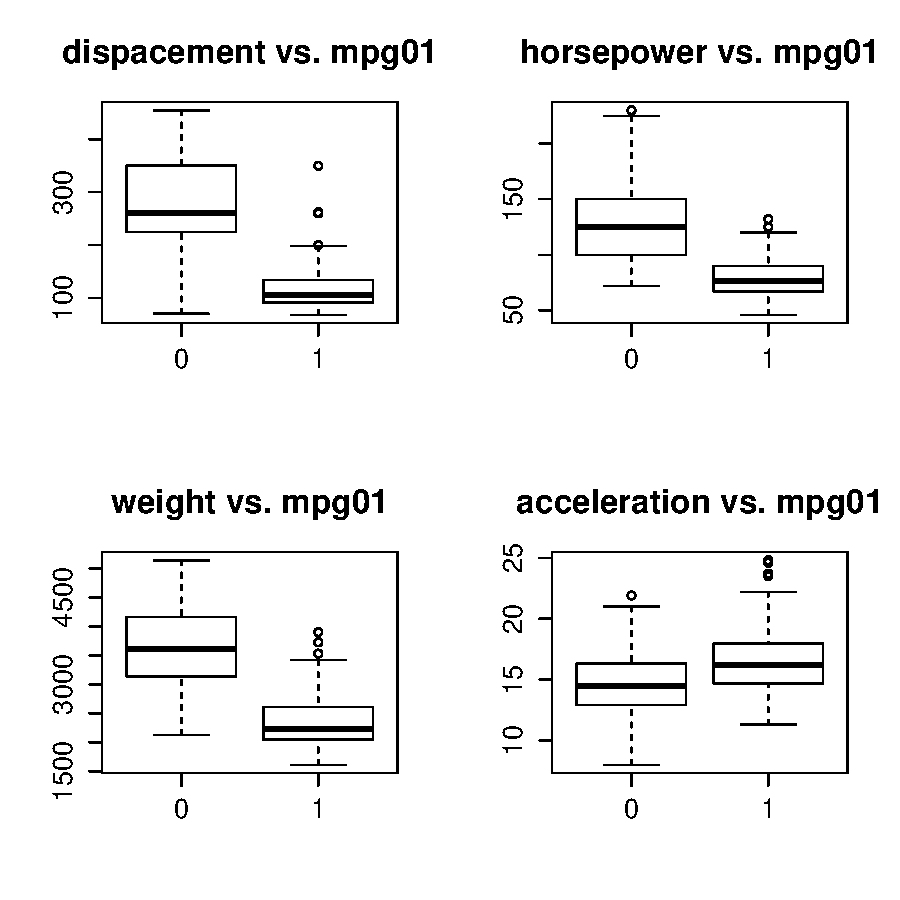
\includegraphics[scale=1]{plot2.pdf}
\end{center}

Weight, displacement, horsepower and year seem most likely to be useful.\\

\item Split the data into a training and a test set.
\begin{lstlisting}
> mask=rep(TRUE,length(mpg01))
> mask[1:length(mask)/2]=FALSE
> mask=sample(mask,length(mask))
> train=Auto01[mask,]
> test=Auto01[!mask,]
> labels.test=mpg01[!mask]
\end{lstlisting}

\item Perform LDA on the training data in order to predict \code{mpg01} using the variables that seemed the most associated with \code{mpg01} in (b).  What is the test error of the model obtained?
\begin{lstlisting}
> lda.fit=lda(mpg01~weight+displacement+horsepower+year, data=Auto01, subset=mask)
> lda.pred=predict(lda.fit, test)
> mean(lda.pred$class==labels.test)
[1] 0.8826531
\end{lstlisting}
The test error rate is $11.73\%$\\

\item Perform QDA on the training data in order to predict \code{mpg01} using the variables that seemed the most associated with \code{mpg01} in (b).  What is the test error of the model obtained?
\begin{lstlisting}
> qda.fit=qda(mpg01~weight+displacement+horsepower+year, data=Auto01, subset=mask)
> qda.pred=predict(qda.fit, test)
> mean(qda.pred$class==labels.test)
[1] 0.8826531
\end{lstlisting}
The test error rate is $11.73\%$\\

\item Perform logistic regression on the training data in order to predict \code{mpg01} using the variables that seemed the most associated with \code{mpg01} in (b).  What is the test error of the model obtained?
\begin{lstlisting}
> glm.fit=glm(mpg01~weight+displacement+horsepower+year, data=Auto01, family=binomial, subset=mask)
> glm.probs=predict(glm.fit, test, type="response")
> glm.pred=rep(0,length(labels.test))
> glm.pred[glm.probs>0.5]=1
> mean(glm.pred==labels.test)
[1] 0.8877551
\end{lstlisting}
The test error rate is $11.22\%$\\

\item Perform KNN on the training data, with several values of $K$, in order to predict \code{mpg01}.  Use only the variables that seemed most associated with \code{mpg01} in (b).  What test errors do you obtain?  Which value of $K$ seems to perform the best on this data set?
\begin{lstlisting}
> train.X=cbind(weight, displacement, horsepower, year)[mask,]
> test.X=cbind(weight, displacement, horsepower, year)[!mask,]
> train.mpg01=mpg01[mask]
> set.seed(1)
> knn.pred1=knn(train.X, test.X,train.mpg01, k=1)
> mean(knn.pred1!=labels.test)
[1] 0.1377551
> set.seed(1)
> knn.pred2=knn(train.X, test.X,train.mpg01, k=5)
> mean(knn.pred2!=labels.test)
[1] 0.09183673
> set.seed(1)
> knn.pred3=knn(train.X, test.X,train.mpg01, k=10)
> mean(knn.pred3!=labels.test)
[1] 0.09183673
> set.seed(1)
> knn.pred4=knn(train.X, test.X,train.mpg01, k=15)
> mean(knn.pred4!=labels.test)
[1] 0.1020408
\end{lstlisting}
A value of $K$ between 5 and 10 seems to perform best on this data.
\end{enumerate}

\item This problem involves writing functions.
\begin{enumerate}
\item Write a function, \code{Power()}, that prints out the result of raising $2$ to the $3$rd power.  In other words, your function should compute $2^3$ and print out the results.
\begin{lstlisting}
> Power=function(){2^3}
> Power()
[1] 8
\end{lstlisting}

\item Create a new function, \code{Power2()}, that allows you to pass any two numbers, \code{x} and \code{a}, and prints out the value of \code{$x^a$}.
\begin{lstlisting}
> Power2=function(x,a){x^a}
> Power2(3,8)
[1] 6561
\end{lstlisting}

\item Using the \code{Power2()} function that you just wrote, compute $10^3$, $8^17$ and $131^3$.
\begin{lstlisting}
> Power2(10,3)
[1] 1000
> Power2(8,17)
[1] 2.2518e+15
> Power2(131,3)
[1] 2248091
\end{lstlisting}

\item Now create a new function, \code{Power3()}, that actually returns the result \code{$x^a$} as an \code{R} object, rather than simply printing it to the screen.
\begin{lstlisting}
> Power3=function(x,a){return(x^a)}
> b=Power3(3,8)
> b
[1] 6561
\end{lstlisting}

\item Now using the \code{Power3()} function, create a plot of $f(x)=x^2$.
\begin{lstlisting}
> plot(x=1:10,y=Power3(1:10,2), main="Graph of f(x)=x^2", xlab="x", ylab="y")
\end{lstlisting}
\begin{center}
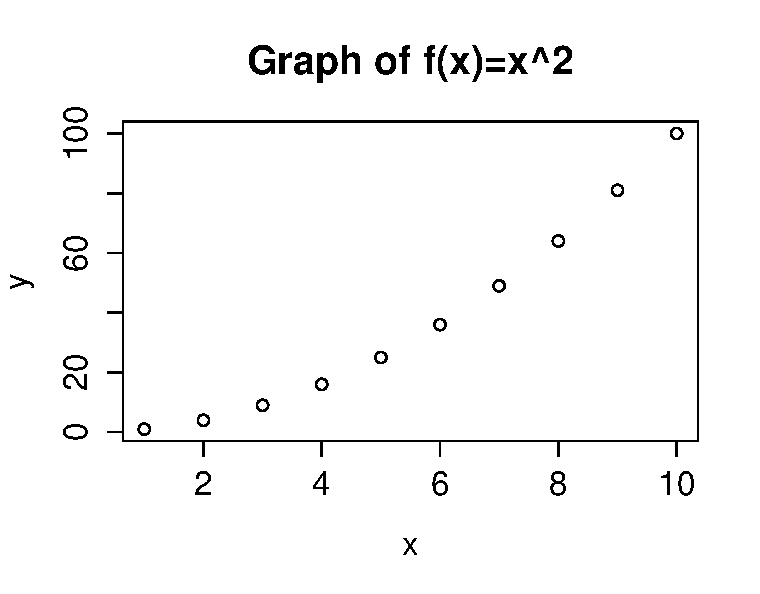
\includegraphics[scale=1]{plot3.pdf}
\end{center}

\item Create a function, \code{PlotPower()}, that allows you to create a plot of \code{x} against \code{$x^a$} for a fixed \code{a} and a range of values of \code{x}.
\begin{lstlisting}
> PowerPlot=function(x,a){plot(x,Power3(x,a), main="Graph of f(x)=x^a", xlab="x", ylab="y")}
> PowerPlot(-10:10,3)
\end{lstlisting}
\begin{center}
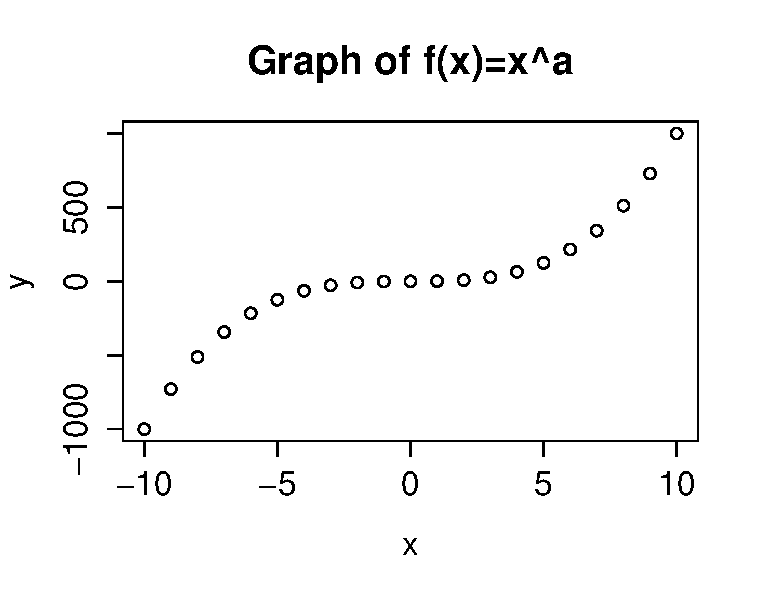
\includegraphics[scale=1]{plot4.pdf}
\end{center}
\end{enumerate}

\item Using the \code{Boston} data set, fit classification models in order to predict whether a given suburb has a crime rate above of below the median.  Explore logistic regression, LDA and KNN models using various subsets of the predictors.  Describe your findings. 
\begin{lstlisting}
> library(MASS)
> attach(Boston)
> crim01=rep(0,length(crim))
> crim01[crim>median(crim)]=1
> Boston01=data.frame(Boston,crim01)
> mask=rep(TRUE,length(crim))
> mask[1:length(mask)/2]=FALSE
> mask=sample(mask,length(mask))
> train=Boston01[mask,]
> test=Boston01[!mask,]
> labels.test=crim01[!mask]
> cor(Boston01[,-4])[14,]
      crim         zn      indus        nox         rm 
 0.4093955 -0.4361510  0.6032602  0.7232348 -0.1563718 
       age        dis        rad        tax    ptratio 
 0.6139399 -0.6163416  0.6197862  0.6087413  0.2535684 
     black      lstat       medv     crim01 
-0.3512109  0.4532627 -0.2630167  1.0000000
\end{lstlisting}

From the correlation matrix it appears that indus, nox, age, dis, rad and tax are most strongly correlated with crim01.  We will use these as the predictors in our models.  We begin with logistic regression.

\begin{lstlisting}
> glm.fit=glm(crim01~indus+nox+age+dis+rad+tax, family=binomial, data=Boston01, subset=mask)
> summary(glm.fit)

Call:
glm(formula = crim01 ~ indus + nox + age + dis + rad + tax, family = binomial, 
    data = Boston01, subset = mask)

Deviance Residuals: 
     Min        1Q    Median        3Q       Max  
-1.89738  -0.27728   0.00038   0.01209   2.48920  

Coefficients:
              Estimate Std. Error z value Pr(>|z|)    
(Intercept) -26.021008   5.317192  -4.894 9.89e-07 ***
indus        -0.066872   0.055810  -1.198  0.23084    
nox          41.763163   9.615915   4.343 1.40e-05 ***
age           0.028577   0.013690   2.087  0.03684 *  
dis           0.414286   0.204815   2.023  0.04310 *  
rad           0.501906   0.168936   2.971  0.00297 ** 
tax          -0.006310   0.003132  -2.014  0.04397 *  
---
Signif. codes:  0 �***� 0.001 �**� 0.01 �*� 0.05 �.� 0.1 � � 1

(Dispersion parameter for binomial family taken to be 1)

    Null deviance: 350.73  on 252  degrees of freedom
Residual deviance: 122.42  on 246  degrees of freedom
AIC: 136.42

Number of Fisher Scoring iterations: 8

> glm.probs=predict(glm.fit, test, type="response")
> glm.pred=rep(0,length(labels.test))
> glm.pred[glm.probs>0.5]=1
> table(glm.pred,labels.test)
        labels.test
glm.pred   0   1
       0 117  13
       1  10 113
> mean(glm.pred==labels.test)
[1] 0.9090909
\end{lstlisting}

The model does quite well with a nearly 91\% test accuracy.  The type I and type II error rates are also comparable.  We now explore LDA.

\begin{lstlisting}
> lda.fit=lda(crim01~indus+nox+age+dis+rad+tax, data=Boston01, subset=mask)
> lda.fit
Call:
lda(crim01 ~ indus + nox + age + dis + rad + tax, data = Boston01, 
    subset = mask)

Prior probabilities of groups:
        0         1 
0.4980237 0.5019763 

Group means:
      indus       nox      age      dis       rad      tax
0  7.195159 0.4730683 50.89127 5.107812  4.253968 309.4683
1 15.598031 0.6472362 87.31969 2.433223 14.834646 511.8110

Coefficients of linear discriminants:
                LD1
indus  0.0073459979
nox    7.3600934820
age    0.0163400220
dis    0.0229312930
rad    0.0737921075
tax   -0.0009765688
> lda.pred=predict(lda.fit, test)
> lda.class=lda.pred$class
> table(lda.class, labels.test)
         labels.test
lda.class   0   1
        0 121  36
        1   6  90
> mean(lda.class==labels.test)
[1] 0.8339921
\end{lstlisting}
LDA performs substantially worse, with only a 83\% test accuracy on the same data.  The rate at which LDA falsely predicts crime to be below the median is substantially higher than for logistic regression. 

\begin{lstlisting}
> library(class)
> train.X=cbind(indus, nox, age, dis, rad, tax)[mask,]
> test.X=cbind(indus, nox, age, dis, rad, tax)[!mask,]
> train.crim01=crim01[mask]
> set.seed(1)
> knn.pred1=knn(train.X, test.X, train.crim01, k=1)
> table(knn.pred1,labels.test)
         labels.test
knn.pred1   0   1
        0 116  12
        1  11 114
> mean(knn.pred1==labels.test)
[1] 0.9090909
> knn.pred2=knn(train.X, test.X, train.crim01, k=5)
> table(knn.pred2,labels.test)
         labels.test
knn.pred2   0   1
        0 107  13
        1  20 113
> mean(knn.pred2==labels.test)
[1] 0.8695652
> knn.pred3=knn(train.X, test.X, train.crim01, k=3)
> table(knn.pred3,labels.test)
         labels.test
knn.pred3   0   1
        0 109  12
        1  18 114
> mean(knn.pred3==labels.test)
[1] 0.8814229
\end{lstlisting}
KNN with $K=1$ also performs quite well on the data, with similar performance to logistic regression. 





%----------------------------------------------------------------------------------------------------------------------------------------
\end{enumerate}
\end{document}